\documentclass[12pt,a4paper]{report}
\usepackage[utf8]{vietnam}\usepackage{amsmath, amsthm, amssymb,latexsym,amscd,amsfonts,enumerate}
\usepackage[top=3.5cm, bottom=3.0cm, left=3cm, right=3.0cm]{geometry} 
\usepackage{color, fancyhdr, graphicx, wrapfig}
\usepackage[unicode]{hyperref}
\usepackage[vietnamese]{babel}
\usepackage{amsthm}
\usepackage{amsmath}
\usepackage{amsfonts}
\usepackage{amssymb}
\usepackage{graphicx} 
\usepackage{titling}
\usepackage{secdot}
\usepackage{enumitem}
\usepackage{tikz}
\usepackage{array}
\usetikzlibrary{calc}
\usepackage{longtable}
\usepackage{indentfirst}
\usepackage{fancyhdr}
\usepackage{exscale,relsize,makeidx}
%\usepackage{refcheck}

\setcounter{tocdepth}{4}
\setcounter{secnumdepth}{4}
\newtheorem{dn}{Định nghĩa}[chapter]
\newtheorem{tc}{Tính chất}[chapter]
\newtheorem{dl}{Định lý}[chapter]
\newtheorem{md}{Mệnh đề}[chapter]
\newtheorem{bd}{Bổ đề}[chapter]
\newtheorem{hq}{Hệ quả}[chapter]
\newtheorem{nx}{Nhận xét}[chapter]
\newtheorem{vd}{Ví dụ}[chapter]
\newtheorem{cy}{Chú ý}[chapter]
\newtheorem{cm}{Chứng minh}[chapter]
\pagenumbering{roman}\pagestyle{plain}
%\pagestyle{fancy}
%\lhead{\it \changefontsizes{11pt}Luận văn thạc sĩ:}
%\rhead{\it Một số phương pháp vô hướng hóa cơ bản trong tối ưu đa mục tiêu}
%\lfoot{\it Nguyễn Văn Vân } 			         
%\rfoot{\it K19.2 trường ĐHSG}
\renewcommand{\headrulewidth}{1,2pt} 			
\renewcommand{\footrulewidth}{1,2pt}

\newcommand{\dstc}[2]
{
	\newdimen\stringwidth\setbox0=\hbox{#1}
	\stringwidth=\wd0
	\hspace*{-\parindent}\hspace*{.5\textwidth}\hspace*{-.5\wd0}#1\hfill #2\bigskip
	
}  
\usepackage{scrextend}
\fancyhf{}
\lhead{}
\chead{\thepage}
\rhead{}
\cfoot{}
\rfoot{}
\lfoot{}
\pagestyle{fancy}
\renewcommand{\headrulewidth}{1pt}

%\changefontsizes{13pt}

\begin{document} 
	\begin{titlepage}
		\begin{tikzpicture}[remember picture, overlay]
			\draw[line width = 1.5pt] ($(current page.north west) + (1in,-1in)$) rectangle ($(current page.south east) + (-0.6in,1in)$);
			
		\end{tikzpicture}
		\centering
		\textbf{ỦY BAN NHÂN DÂN THÀNH PHỐ HỒ CHÍ MINH\smallskip\\
			TRƯỜNG ĐẠI HỌC SÀI GÒN}\par
		\rule{5cm}{0.5pt}\par
		\vspace{2cm}
		{\Large\textbf{ĐỖ NGỌC MINH THƯ \\ NGUYỄN CHÍ BẰNG}\par}
		\vspace{4cm}
		{\Large\textbf{PHƯƠNG PHÁP GIẢI BÀI TOÁN\\ TỐI ƯU TUYẾN TÍNH NGUYÊN }\par}
		\vspace{4cm}
		\large\textbf{ ĐỀ TÀI NGHIÊN CỨU KHOA HỌC SINH VIÊN}\par		
		
		\large{CHUYÊN NGÀNH: TOÁN ỨNG DỤNG}
		\vspace{1.5cm}
		
		\vfill
		\textbf{Thành phố Hồ Chí Minh, năm 2021}
	\end{titlepage}
	\begin{titlingpage}
		\begin{tikzpicture}[remember picture, overlay]
			\draw[line width = 1.5pt] ($(current page.north west) + (1in,-1in)$) rectangle ($(current page.south east) + (-1in,1in)$);
			
		\end{tikzpicture}
		\centering
		\textbf{ỦY BAN NHÂN DÂN THÀNH PHỐ HỒ CHÍ MINH\smallskip\\
			TRƯỜNG ĐẠI HỌC SÀI GÒN}\par
		\rule{5cm}{0.5pt}\par
		\vspace{2cm}
		{\Large\textbf{ĐỖ NGỌC MINH THƯ \\ NGUYỄN CHÍ BẰNG}\par}
		\vspace{4cm}
		{\Large\textbf{PHƯƠNG PHÁP GIẢI BÀI TOÁN \\ TỐI ƯU TUYẾN TÍNH NGUYÊN}\par}
		\vspace{4cm}
		\large\textbf{ĐỀ TÀI NGHIÊN CỨU KHOA HỌC SINH VIÊN}\par		
		
		\large{CHUYÊN NGÀNH: TOÁN ỨNG DỤNG}
		\vspace{1.5cm}
		
		\large\textbf{Người hướng dẫn} \par
		\vspace{2cm}
		
		\large\textbf{PGS.TS. TẠ QUANG SƠN}\par
		
		%	\includegraphics[height=2cm]{chukynew}
		\vfill
		\textbf{Thành phố Hồ Chí Minh, năm 2021}
	\end{titlingpage}
	
	%\large
	\renewcommand{\baselinestretch}{1.2}
	\fontsize{13pt}{20pt}\selectfont
	
	\chapter*{Lời cam đoan}
	\thispagestyle{fancy}
	\addcontentsline{toc}{chapter}{Lời cam đoan}
	\vspace{1cm}
	\indent
	
	Chúng tôi tên là Đỗ Ngọc Minh Thư và Nguyễn Chí Bằng, là các  sinh viên lớp DTU1221, khoa Toán - Ứng dụng , khóa 2022-2026,  thuộc trường Đại học Sài Gòn. 
	Xin cam đoan rằng: Toàn bộ nội dung được trình bày trong đề tài  này này đều do chúng tôi thực hiện dưới sự hướng dẫn của PGS.TS. Tạ Quang Sơn.
	Những kết quả nghiên cứu của tác giả khác được sử dụng trong đề tài  đều có trích dẫn đầy đủ. 
	Chúng tôi xin chịu trách nhiệm nếu có các nội dung sao chép không hợp lệ hoặc vi phạm quy chế đào tạo. 
	\\
	\\
	\\
	\rightline{{\it {Tp. HCM, tháng ... năm 2024}} \hspace*{0cm}}
	\rightline{\textbf{Tác giả} \hspace*{2cm}}
	\\
	\\
	\\
	
	%\vspace*{1cm}
	\rightline{\textbf{Đỗ Ngọc Minh Thư}\hspace*{0.75cm}}
	
	\chapter*{Lời cảm ơn}
	\thispagestyle{fancy}
	\addcontentsline{toc}{chapter}{Lời cảm ơn}
	\vspace{1cm}
	\indent
	
	Đề tài nghiên cứu khoa học này được hoàn thành tại trường Đại Học Sài Gòn dưới sự hướng dẫn của PGS.TS. Tạ Quang Sơn. Chúng em xin bày tỏ sự kính trọng cùng lòng biết ơn chân thành và sâu sắc với Thầy. Sự tận tâm và nhiệt tình hướng dẫn của Thầy đã giúp chúng em nâng cao hiểu biết và hoàn thành đề tài nghiên cứu khoa học này.
	
	
	\bigskip
	Xin cám ơn Phòng Đào tạo  và Khoa Toán - Ứng dụng, Trường Đại học Sài Gòn, đã tạo nhiều điều kiện thuận lợi, hỗ trợ giúp chúng em nâng cao chất lượng và nhiệm vụ học tập qua việc thực hiện đề tài này.
	\\
	\\
	\\
	\rightline{{\it {Tp. HCM, tháng ... năm 2024}} \hspace*{0cm}}
	\rightline{\textbf{Tác giả} \hspace*{2cm}}
	\\
	\\
	
	\vspace{1cm}
	\rightline{\textbf{Đỗ Ngọc Minh Thư} \hspace*{0.75cm}}
	\newpage
	
	\addcontentsline{toc}{chapter}{Mục lục}
	\tableofcontents
	%\thispagestyle{plain}
	\chapter*{Danh mục các kí hiệu}
	\thispagestyle{fancy}
	\addcontentsline{toc}{chapter}{Danh mục các kí hiệu}
	\begin{longtable}{l l}
		
		$\mathbb{R}$ & Tập các số thực\\
		%$\emptyset $ & Tập rỗng\\
		$\mathbb{R}^n$ & Không gian Euclide $n$-chiều\\

		
		$F$ & Tập chấp nhận được của bài toán tối ưu\\
		$\langle u, v \rangle$ & Tích vô hướng của hai véc tơ $u$ và $v$ trong $\mathbb{R}^n$\\
		
		
	\end{longtable}
\newpage
\pagenumbering{arabic} 
\chapter*{Lời nói đầu}
\thispagestyle{fancy}
\addcontentsline{toc}{chapter}{{\bf  Lời nói đầu}\rm}
\renewcommand{\baselinestretch}{1.2}
Thực tế cho thấy rằng trong nhiều bài toán tối ưu, nghiệm tìm được mong muốn phải là các số nguyên hoặc một bộ phận nghiệm của bài toán phải là các số nguyên. Điều này có thể thấy ở các bài toán như phân phối hàng hóa, sắp xếp tối ưu nhân lực, bài toán trên mạng, phân luồng giao thông,...\\
Đã từng có nhận định về việc tìm nghiệm nguyên của bài toán tối ưu là sau khi tìm được nghiệm tối ưu thì thưc hiện việc làm tròn nghiệm. Cách thức này thường không cho kết quả như mong muốn. Bởi lẽ nghiệm làm tròn có thể không thuộc miền chấp nhận được hoặc  có thể việc làm tròn như thế không chắc đã cho nghiệm tốt nhất như mong muốn. Lý thuyết về việc tìm nghiệm nguyên cho các bài toán tối ưu đáp ứng điều mong đợi nêu trên.

Bài toán tối ưu thường được xem xét dưới dạng 
$$
\begin{array}{ll}
{\rm Min\ (Max)}& f(x)\\
&x \in F,
\end{array}
$$
trong đó $f(x)$ là hàm mục tiêu tối ưu cần xác định, phụ thuộc vào biến $x$, xác định trên một không gian cho trước và $F$ là tập ràng buộc còn gọi là tập chấp nhận được. Mục tiêu của bài toán là đi tìm $x\in F$ sao cho hàm mục tiêu $f(x)$ đạt giá trị lớn nhất hay bé nhất.
Vì bài toán Max có thể đưa về bài toán Min và ngược lại, nên trong nhiều trường hợp để xây dựng các thuật toán tìm nghiệm cho bài toán, người ta chỉ cần xét một trong hai dạng nêu trên là đủ.



Trong đề tài này chúng tôi quan tâm tìm hiểu về nghiệm nguyên cho bài toán có hàm mục tiêu tuyến tính trên tập chấp nhận được xác định bởi các hàm tuyến tính. Bài toán có dạng như sau
$$
\begin{array}{ll}
{\rm Min}&\quad c_1x_1+\ldots+c_nx_n\\
{\rm s.t.}&\begin{cases}
a_{11}x_1+\ldots+a_{1n}x_n \le b_1\\
a_{21}x_1+\ldots+a_{2n}x_n \le b_2\\
\vdots\\
a_{m1}x_1+\ldots+a_{mn}x_n \le b_m\\
x_1, \ldots, x_n \ge 0.
\end{cases}
\end{array}
$$
Trong đó, $c_i, i=1,...,n$, các hệ số $a_{ij}$ với $i=1,...,m$ và $j=1,...,n$, và $b_i$ với $i=1,...,m$ là các số thực cho trước.

Bằng cách dùng ký hiệu véc tơ và ma trận, bài toán nêu trên được viết dưới dạng 
$$
\begin{array}{rl}
{\rm Min}& \langle c,x \rangle \\
{\rm s.t.}& 
\begin{cases}Ax \le b\\
 x\ge 0.
 \end{cases}
\end{array}
$$
Trong đó, cho trước $A$ là ma trận có $m$ dòng và $n$ cột, $c$ là véc tơ $n$ chiều và $b$ là véc tơ $m$ chiều. Chú ý rằng, các ràng buộc bất đẳng thức đều có thể biến đổi về ràng buộc đẳng thức. Vì thế trong nội dung của đề tài này, nếu không nói gì thêm, bài toán luôn được xét dưới dạng tổng quát
$$
\begin{array}{rl}
{\rm (IP) \; Min}& \langle c,x \rangle \\
{\rm s.t.}& 
\begin{cases}Ax = b\\
 x\ge 0.
 \end{cases}
\end{array}
$$

Các phương pháp mà đề tài này tìm hiểu là phương pháp sử dụng siêu phẳng cắt Gomory và phương pháp tìm nghiệm nguyên theo kiểu nhánh-cận do Land-Doig đề xuất. 

Nội dung đề tài được tổ chức thành 3 chương trong đó 

Chương 1; Dành để tóm lược lại một số kiến thức về Đại số tuyến tính liên quan đến véc tơ và ma trận. Đồng thời chương này cũng nhắc lại một số kết quả về phương pháp đơn hình khi giải bài toán quy hoạch tuyến tính.

Chương 2: Là phần chính của nội dung đề tài. Trong đó được chia làm hai phần. Phần đầu dành để trình bày phương pháp dùng siêu phẳng cắt Gomory và phần tiếp theo dành để trình bày phương pháp nhánh-cận kiểu Land-Doig. Trong mỗi phần đều có các ví dụ minh họa. Ngoài ra, dựa trên thực tế, khi sử dụng các phương pháp này để giải bài toán Quy hoạch nguyên, đề tài cũng đưa ra những nhận xét về phương pháp.

Phần cuối của đề tài này là Chương 3. Chúng tôi thử áp dụng các phương pháp trên để khảo sát việc tìm nghiệm nguyên cho bài toán dạng phân thức tuyến tính. 

Do lần đầu tham gia tập dượt nghiên cứu khoa học. Các tri thức chọn lọc và trình bày trong nội dung của đề tài này chưa đầy đủ hoặc còn sơ suất. Chúng em kính mong nhận được sự chỉ bảo từ quý thầy cô.

\newpage
\renewcommand{\baselinestretch}{1.2}
 
\chapter{Một số kiến thức cơ bản về bài toán quy hoạch tuyến tính} 
Kiến thức trình bày trong chương này, hầu hết được tham khảo từ các tài liệu  \cite{xxx} và \cite{xxx}.

\section{Một số kiến thức cơ bản về Bài toán tối ưu tuyến tính}

\subsection{Bài toán dạng chính tắc và chuẩn tắc}
\begin{itemize}
    \item \textbf{Bài toán dạng chính tắc}
    
    Ta có bài toán dạng:
    \begin{equation} \small \label{F}
        \begin{split}
        f(x) & = c^Tx \quad \longrightarrow \text{Min} \\
            & \left\{
            \begin{split}
            & \sum _{j=1}^n a_{ij} x_j = b_i, \: i=1,2,\ldots,m \\
            & x_j \geq 0, \: j=1,2,\ldots,n.
            \end{split}
            \right.    
        \end{split}
    \end{equation}

    Thì ta gọi bài toán trên có dạng chính tắc và có thể viết lại dưới dạng:

    \begin{equation} \small \label{chinhtac}
        \begin{split}
        (P) \quad \text{Min } & f(x) = c^Tx \\
            & \left\{
            \begin{split}
            & Ax=b, \\
            & x_j \geq 0.
            \end{split}
            \right.    
        \end{split}
    \end{equation}

    Trong đó $A$ là ma trận $m\times n$, $b=\begin{pmatrix}
        b_1 \\
        b_2 \\
        \vdots \\
        b_m
        \end{pmatrix}$ và $c^T=(c_1 \: c_2 \: \ldots \: c_n)$.

    \item \textbf{Bài toán dạng chuẩn tắc}
    
    Nếu bài toán có dạng:

    \begin{equation} \small \label{F}
        \begin{split}
        f(x) & = c^Tx \quad \longrightarrow \text{Min} \\
            & \left\{
            \begin{split}
            & \sum _{j=1}^n a_{ij} x_j \geq b_i, \: i=1,2,\ldots,m \\
            & x_j \geq 0, \: j=1,2,\ldots,n.
            \end{split}
            \right.    
        \end{split}
    \end{equation}

    Thì ta gọi bài toán trên có dạng chuẩn tắc và có thể viết lại dưới dạng:

    \begin{equation} \small \label{F}
        \begin{split}
        (P) \quad \text{Min } & f(x) = c^Tx \\
            & \left\{
            \begin{split}
            & Ax \geq b, \\
            & x_j \geq 0.
            \end{split}
            \right.    
        \end{split}
    \end{equation}

    Tương tự $A$ là ma trận $m\times n$, $b=\begin{pmatrix}
        b_1 \\
        b_2 \\
        \vdots \\
        b_m
        \end{pmatrix}$ và $c^T=(c_1 \: c_2 \: \ldots \: c_n)$.

\end{itemize}

\subsection{Chuyển bài toán về dạng chính tắc}

Để thuận tiện, ta chỉ xét dạng bài toán quy hoạch tuyến tính tổng quát là \textbf{dạng chính tắc} và bất kỳ bài toán nào cũng có thể đưa về dạng chính tắc.

\begin{itemize}
\item \textbf{Phương pháp đưa về dạng chính tắc:}
    \begin{itemize}
    \item Bài toán $\max f(x) \longrightarrow -\min [-f(x)]$.
    \item Bằng cách thêm ẩn phụ $x_{n+i}$ tương ứng có hệ số trong hàm mục tiêu là $c_{n+i}=0$, ta có thể đưa bất đẳng thức 
    \begin{equation*}
    \sum _{j=1}^n a_{ij} x_j \geq b_i
    \end{equation*}
    hoặc
    \begin{equation*}
    \sum _{j=1}^n a_{ij} x_j \leq b_i
    \end{equation*}
    lần lượt thành đẳng thức
    \begin{equation*}
    \sum _{j=1}^n a_{ij} x_j - x_{n+i} = b_i
    \end{equation*}
    hoặc
    \begin{equation*}
    \sum _{j=1}^n a_{ij} x_j + x_{n+i} = b_i
    \end{equation*}
    \item Nếu tồn tại bất kỳ $x_k$ không có ràng buộc thì ta viết
    \begin{equation*}
    x_k = x_k^{'} - x_k^{''}
    \end{equation*}
    với $x_k^{'} \geq 0$ và $x_k^{''} \geq 0$.
    \end{itemize}
\end{itemize}
Kể từ đây, ta chỉ quan tâm bài toán \eqref{chinhtac}.

\section{Phương pháp giải bài toán tối ưu tuyến tính}

\subsection{Phương pháp hình học}

\subsection{Phương pháp đơn hình}
























\subsection{Phương pháp đơn hình đối ngẫu}
\subsubsection{ Bài toán đối ngẫu }
\begin{itemize}
    \item \textbf{Bài toán gốc và bài toán đối ngẫu dạng chuẩn tắc:}\\
    Xét hai bài toán sau:\\
    \begin{minipage}[t]{0.48\linewidth}
   \begin{equation}\label{baitoangoc}
     \begin{split}
          & {\rm{Min}} \langle c,x \rangle\\
          \rm{s.t} &\left\{\begin{split}
            & Ax\ge b,\\
            & x \ge 0.\\
           \end{split}\right.
       \end{split}
   \end{equation}
\end{minipage}\hfill
\begin{minipage}[t]{0.48\linewidth}
\begin{equation}\label{baitoandoingau}
    \begin{split}
        & {\rm{Max}} \langle b,y \rangle\\
       \rm{s.t} & \left\{\begin{split}
            &A^Ty \le c,\\
            & y\ge 0.\\
        \end{split}\right.
    \end{split}
\end{equation}
\end{minipage}
\begin{dn}
    Cho bài toán QHTT dạng chuẩn \eqref{baitoangoc} và bài toán \eqref{baitoandoingau} được gọi là các \textbf{bài toán đối ngẫu } (hay còn gọi là \textbf{cặp đối ngẫu}).\\
\end{dn}
Bài toán \eqref{baitoangoc} gọi là \textit{bài toán gốc}, bài toán \eqref{baitoandoingau} gọi là bài toán đối ngẫu.\\
Trong phần này ta luôn xét bài toán Min cho bài toán gốc và bài toán Max cho bài toán đối ngẫu.\\
  \item \textbf{Bài toán gốc và bài toán đối ngẫu dạng chỉnh tắc:}\\
      \begin{minipage}[t]{0.48\linewidth}
    Bài toán gốc
   \begin{equation}
       \begin{split}
           &{\rm{Min }} \langle c,x \rangle\\
          \rm{s.t} &\left\{\begin{split}
            & Ax= b\\
            & x \ge 0\\
           \end{split}\right.
       \end{split}
   \end{equation}
\end{minipage}\hfill
\begin{minipage}[t]{0.48\linewidth}
Bài toán đối ngẫu
\begin{equation}
    \begin{split}
        &{\rm{Max}} \langle b,y \rangle\\
       \rm{s.t} & \left\{\begin{split}
            & A^Ty \le (\ge) c\\
            & y \hspace{0.1cm1cm} \text{tự do}\\
        \end{split}\right.
    \end{split}
\end{equation}
\end{minipage}
\item\textbf{Các tính chất của cặp bài toán đối ngẫu}
\begin{dl}\label{doingauyeu}
(Đối ngẫu yếu) Nếu $x$ là một phương án bất kì của bài toán gốc \eqref{baitoangoc} và $y$ là phương án là một phương án bất kì của bài toán đối ngẫu \eqref{baitoandoingau} thì $f(x)\ge g(y) $.
    \end{dl}
   
    \begin{dl}
        Nếu $x^*$ là phương án bất kì của bài toán gốc \eqref{baitoangoc} và $y^*$ là phương án bất kì của bài toán đối ngẫu (\eqref{baitoandoingau} và có $f(x^*)=g(y^*)$ thì $x^*$ là phương án tối ưu của bài toán gốc \eqref{baitoangoc} và $y^*$ là phương án tối ưu của bài toán đối ngẫu \eqref{baitoandoingau}.\\
    \end{dl}

\begin{dl}
        (Đối ngẫu mạnh) \\
      a) Nếu bài toán gốc có phương án tối ưu $x^*$ thì bài toán đối ngẫu cũng có phương án tối ưu $y^*$ và ngược lại, đồng thời $f(x^*)=g(y^*)$.\\
      b) Nếu hàm mục tiêu của bài toán gốc không bị chặn dưới thì bài toán đối ngẫu không có phương án.\\
        Nếu hàm mục tiêu của bài toán đối ngẫu không bị chặn trên thì bài toán gốc không có phương án .
    \end{dl}

\begin{hq}
        Đối với mỗi cặp bài toán quy hoạch đối ngẫu chỉ có thể xảy ra một trong ba khả năng loại trừ nhau sau đây:\\
        a) Bài toán gốc và bài toán đối ngẫu đều không có phương án.\\
        b) Bài toán gốc và bài toán đối ngẫu đều có phương. Khi đó cả hai bài toán đều có phương án tối ưu và giá trị tối ưu hàm mục tiêu của hai bài toán là bằng nhau.\\
        c) Một bài toán có phương án và bài toán còn lại không có phương án. Khi đó, bài toán có phương án sẽ không có phương án tối ưu và hàm mục tiêu của bài toán đó không bị chặn trong miền ràng buộc.
    \end{hq}
    \begin{hq}
        Điều kiện cần và đủ để cặp phương án tối ưu $x^*,y^*$ là phương án tối ưu của cặp bài toán đối ngẫu \eqref{baitoangoc},\eqref{baitoandoingau} là $c^Tx^*=b^Ty^*$.
    \end{hq}
    \begin{dl}
        (Độ lệch bù yếu) Giả sử $x \in R^n$ là phương án của bài toán gốc \eqref{baitoangoc}, $y\in R^m$ là phương án tối ưu của bài toán đối ngẫu \eqref{baitoandoingau}. Khi đó, điều kiện cần và đủ để $x$ và $y$ là phương án tối ưu của các bài toán tương ứng là :\\
        i) $(a_{i1}x_ +a_{in}x_n -b_i)y_i=0 (\forall {i=1,..m}) $ \\
        ii) $(c_j-(a_{1j} y_1+...a_{mj}y_m))x_j=0 (\forall{j=1,..n}) $ \\   
    \end{dl}
    Nếu biết phương án tối ưu của bài toán gốc, vận dụng lý thuyết đối ngẫu ta có thể suy ra phương án tối ưu của bài toán đối ngẫu tương ứng mà không cần giải nó.\\
    \textbf{\textit{Chú ý:}} \\
    Điều kiện i của định lý (1.4) cho ta kết quả:\\
        - Nếu $y_i \ge 0 $ thì $\sum_{j=1}^n a_{in}x_n=b_i.$\\
        - Nếu $\sum_{j=1}^n a_{in}x_n >b_i$ thì $y_i=0$.\\ 
    Điều kiện (1.4.2) cho ta kết quả:\\
        - Nếu $x_j \ge 0$ thì $\sum_{i=1}^m a_{mj}y_m=c_j.$\\
        - Nếu $\sum_{i=1}^m a_{mj}y_m<c_j$ thì $x_j=0$.\\
    \end{itemize}
    \textit{Nhắc lại} Ràng buộc chặt là ràng buộc xảy ra dấu =. Ràng buộc lỏng là ràng buộc xảy ra dấu bất đẳng thức thực.\\
    Định lý độ lệch bù yếu còn có thể phát biểu lại như sau:\\
    $x^*,y^*$ là phương án tối ưu của bài toán gốc và bài toán đối ngẫu khi và chỉ khi $x^*,y^*$ là phương án của bài toán tương ứng và thỏa mãn điều kiện nếu một ràng buộc là lỏng (tức là bị lệch) thì ràng buộc đối ngẫu tương ứng với nó phải chặt (tức là bù lại ).\\
    \begin{bd}
        Đối với một cặp bài toán đối ngẫu, nếu một ràng buộc là lỏng đối với đối với một phương án tối ưu của bài toán này thì ràng buộc đối ngẫu của nó phải chặt đối với phương án tối ưu của bài toán kia.\\
    \end{bd}
     \begin{dl}
        (Độ lệch bù mạnh) Nếu cặp bài toán đối ngẫu có phương án tối ưu thì tồn tại một cặp phương án tối ưu thỏa mãn điều kiện nếu một ràng buộc là chặt thì ràng buộc đối ngẫu của nó phải là lỏng.\\
        
    \end{dl}
\subsubsection{Phương pháp đơn hình đối ngẫu:}
\begin{itemize}
    \item \textbf{Cơ sở chấp nhận được đối ngẫu:}\\
    \begin{equation}\label{chapnhan}
     \begin{split}
          & {\rm{Min}} \langle c,x \rangle\\
          \rm{s.t} &\left\{\begin{split}
            & Ax= b,\\
            & x \ge 0.\\
           \end{split}\right.
       \end{split}
   \end{equation}
    Giả thiết rank $A=m$. Giả sử, $\{A_j|j\in J\} $ là hệ $m$ vecto độc lập tuyến tính của A, gọi là hệ vecto cơ sở. J là tập chỉ số cơ sở. Ký hiệu $A_j$ lập nên từ các véc  cơ sở, gọi là ma trận cơ sở.\\
    Ký hiệu $H=\{1,2,...,n\} \setminus J $. Phương án cơ sở $(x_J,x_H)$ của bài toán \eqref{chapnhan} tương ứng với cơ sở $J$.
    \begin{dn}
        a) Ta gọi cơ sở $J$ là\textit{ chấp nhận được gốc} nếu phương án cơ sở tương ứng với nó là phương án chấp nhận được.\\
        b) Nếu phương án cơ sở tương ứng với $J$ là phương án tối ưu thì $J$ sẽ gọi là \textit{cơ sở tối ưu}.\\
    \end{dn}
    Xét bài toán đối ngẫu với bài toán \eqref{chapnhan}
    \begin{equation}\label{doingauchapnhandoingauchapnhan}
    \begin{split}
        & {\rm{Max}} \langle b,y \rangle\\
       \rm{s.t} & \left\{\begin{split}
            &A^Ty \le c,\\
            & y \hspace{0.1cm}\text{tự do}\\
        \end{split}\right.
    \end{split}
\end{equation}
\begin{dn}
        a) Ta gọi phương án \textit{ cơ sở đối ngẫu} tương ứng với cơ sở J là vecto $y$ thu được bằng cách giải hệ phương trình tuyến tính $A^T_J y=c_J$ (nghĩa là $y=(A^T_J)^{-1}c_J$).\\
        b) Cơ sở J được gọi là \textit{cơ sở chấp nhận được đối ngẫu} nếu phương án cơ sở đối ngẫu ứng với nó là phương án chấp nhận được của bài toán đối ngẫu.
    \end{dn}
    Nếu $J$ là cơ sở chấp nhận được đối ngẫu thì phương án cơ sở đối ngẫu tương ứng $y=(A^T_J)^{-1}c_J$ phải thỏa mãn ràng buộc $A^Ty\le c$, nghĩa là $$A^T(A^T_J)^{-1}c_J-c \le 0$$.\\
    Ta xét $z^k$ từ biểu diễn $A^T=z^kA^T_J$, hay $z^k=A^T(A^T_J)^{-1}$.\\
    Vậy $J$ là cơ sở chấp nhận được đối ngẫu nếu $z_Hc_J-c\le 0$, hay  $\sum_{j\in J}z_{jk}c_j-c_k\le 0 (\forall k \notin J)$ và $=0$ nếu $k\in J$. Đây là tiêu chuẩn tối ưu của cơ sở $J$. Ta suy ra khẳng định sau đây.\\
    \begin{md}
        Nếu cơ sở $J$ vừa chấp nhận được gốc vừa chấp nhận được đối ngẫu, thì nó là cơ sở tối ưu của bài toán gốc.
    \end{md}
    \item \textbf{Thuật toán đơn hình đối ngẫu}
    Giả sử J là cơ sở chấp nhận được đối ngẫu. Giả thiết rằng $J=\{1,2,...,m\}$. Ta lập bảng giống như bảng đơn hình cho bài toán gốc với cơ sở J.\\
    \begin{tabular}{|c|c|c|c|c|c|c|c|c|}
       \hline
       Cơ sở  & Hệ số& Giả PA& $x_1$ &$x_2$ & \ldots &$x_k$ &\ldots &$x_n$  \\
       \hline
        $x_J$ & $c_J$ &$x_J^0$ & $c_1$ & $c_2$ & \ldots &$c_k$ &\ldots &$c_n$\\
        $x_1$ & $c_1$ & $x_1$ &$z_{11}$ & $z_{12}$ &\ldots &$z_{1k}$ &\ldots &$c_{1n}$\\
        $x_2$ &$c_2$ &$x_2$ &$z_{21}$ &$z_{22}$ & \ldots &$z_{2k}$ & \ldots &$z_{2n}$\\
        \vdots&\vdots & \vdots & \vdots &\vdots & \vdots &\vdots &\vdots & \vdots \\
        $x_m$ &$c_m$ &$x_m$ &$z_{m1}$ &$z_{m2}$ &\ldots &$z_{mk}$ &\ldots &$z_{mn}$\\
        \hline
        && $f(x)$ & $\Delta_1$ &$\Delta_2$ &\ldots &$\Delta_k$ & \ldots & $\Delta_n$\\
        \hline
        
    \end{tabular}\\
    Ý nghĩa của các ký hiệu giống như là bảng đơn hình. Chỉ có cột giả phương án là khác, cột này được lấy từ hệ thống \\
    $$x_0^J=A_J^{-1}b$$\\
    Lưu ý hàng ước lượng $\Delta_k$ đề không dương vì giả thiết $J$ là cơ sở chấp nhận được đối ngẫu.\\ 
    Giả sử bài toán luôn có cơ sở đối ngẫu chấp nhận được, ta có các bước thuật toán.\\
    \textbf{\textit{THUẬT TOÁN:}}\\
    \textbf{Bước 1} Tìm giải phương án $J,A_J, A_J^{-1}$, giả phương án án $x_J^0,Z_J.$\\
    \textbf{Bước 2} (Kiếm tra tiêu chuẩn tối ưu)\\
    Cơ sở đang xét sẽ là tối ưu nếu mọi thành phần $x_j$ của cột giả phương án đều $x_J \ge 0$.Vì khi đó nó là cơ sở chấp nhận được gốc vì thế tối ưu.\\
    a) Nếu $x_j\ge 0, \forall j \in J$ thì giả phương án ($x_J,x_H$) là phương án tối ưu, thuật toán dừng.\\
    b) Nếu tồn tại $j \in J$ mà $x_j <0 $ thì ta chọn chỉ số r ứng với \textbf{$x_r=min \{x_j, j \in J\}$}.\\ 
    \textbf{Bước 3} Kiểm tra điều kiện để tập phương án khác rỗng.\\
    a) Nếu có dòng ứng với $x_j <0 (j \in J)$ mà $z_{jk}\ge 0 $ với mọi $k=1,2..,n$.\\
    b)Nếu trên mỗi dòng ứng với $x_j <0$ đều tìm được ít nhất một phần tử $z_{jk} <0$.Khi đó ta tiến hành một bước lặp đơn hình.\\
    Tìm cột xoay thỏa mãn $\dfrac{\Delta_s}{z_{rs}}=min \{\dfrac{\Delta_j}{z_{rj}}; z_{rj} <0\}$.\\
    \textbf{Bước 4} Thực hiện xoay hàng và cột để thiết lập bảng đơn hình mới. Cách làm giống như cách làm phương pháp đơn hình.\\
    Lặp lại bước 2.
    \textbf{Ví dụ }
         Giải bài toán quy hoạch tuyến tính chuẩn tắc\\
    \begin{equation*}
        \begin{split}
            &f(x)=15x_1+12x_2+10x_3 \longrightarrow min\\
            & \left\{\begin{split}
                &3x_1+4x_2+2x_3 \ge 160\\
                &x_1 +2x_2 +3 x_3 \ge 140\\
                & x_1,x_2,x_3 \ge 0 \\
            \end{split}\right.
        \end{split}
    \end{equation*}
    Ta đưa bài toán về dạng chính tắc và đổi dấu hai vế ràng buộc đẳng thức.
    Ta nhận được bài toán như sau:\\
    \begin{equation*}
        \begin{split}
            &f(x)=15x_1+12x_2+10x_3 \longrightarrow min\\
            & \left\{\begin{split}
                &-3x_1-4x_2-2x_3 +x_4 = 160\\
                &-x_1 -2x_2 -3x_3 
 +x_5 = 140\\
                & x_1,x_2,x_3,x_4,x_5 \ge 0 \\
            \end{split}\right.
        \end{split}
    \end{equation*}
    Từ đây ta có được giả phương án ban đầu là $x^0=(0,0,0,-160,-140)^T,\\  
   f_0=f(x^0)=0$.

    Ta lập được bảng đơn hình sau:\\
    \begin{tabular}{|c|c|c|c|c|c|c|c|}
       \hline
       Cơ sở  & Hệ số & Giả PA& $x_1$ & $x_2$ & $x_3$ &$x_4$ & $x_5$ \\
       \hline
        $x_J$ & $c_J$ & $x_J^0$ & $15$ &$12$ &$10$ &$0$ &$0$ \\
        \hline
        $x_4$ & $0$ & $-160^*$ & $-3$ &$-4^*$ &$-2$ &$1$ &$0$\\
        $x_5$ & $0$ & $-140$ &$-1$ &$-2$ &$-3$ &$0$ &$1$\\
        \hline
        &Bảng 1 & $0$ & $-15$ &$-12$ &$-10$ &$0$ &$0$\\
        \hline
        $x_2$& $12$ &$40$ & $3/4$ &$1$ &$1/2$ &$-1/4$ &$0$\\
        $x_5$ &$0$ & $-60$ &$1/2$ &$0$ &$-2^*$ &$-1/2$ &$1$\\
        \hline
        &Bảng 2& $480$ &$-6$ &$0$ &$-4$ &$-3$ &$0$\\
        \hline
        $x_2$ &$12$ &$25$ &$7/8$ & $1$ &$0$ &$0 $ &$0$\\
        $x_3$ &$10$ &$30$ &$-1/4$ &$0$ &$1$ &$1/4$ &$-1/2$\\
        \hline
        &Bảng 3& $600$ &$-7$ &$0 $ &$0$ &$-2$ &$-2$\\
        \hline
    \end{tabular}\\
      Trong bảng 1, cột giả phương án có phần tử âm, nên ta chưa nhận được phương án tối ưu. Ta chọn dòng $x_4$  ( tương ứng với số âm nhỏ nhất $-160$) làm dòng quay. Cột quay là cột $x_2$ (tương ứng với số âm nhỏ nhất trong ba tỉ số $\frac{-15}{3},\frac{-12}{-4},\frac{-10}{-2}$). Phần tử quay bằng $-4$. Biến đổi bảng này theo quy tắc đơn hình ta nhận được Bảng 2.\\
    Trong Bảng 2,cột giả phương án vẫn còn phần tử âm. Ta chọn dòng $x_5$ làm dòng quay và chọn cột $x_3$ làm cột quay. Lúc này phần tử quay là $-2$. Ta tiếp tục biến đổi bảng đơn hình và nhận được Bảng 3. \\
    Ở Bảng 3, mọi phần tử trong cột giả phương án đều dương nên ta nhận được phương án tối ưu: $x^*=(0,25,30)^T$ với $f_{\rm{min}}=600$.\\
    
\end{itemize}





























\chapter{Bài toán tối ưu tuyến tính có nghiệm nguyên}
Thực tế hiện nay cho thấy rằng việc tìm kết quả của các bài toán tối ưu tuyến tính với các biến ràng buộc là số thực là chưa đủ. Nhiều bài toán Quy hoạch tuyến tính đòi hỏi phải tìm được nghiệm là các biến nguyên, được gọi là mô hình tối ưu tuyến tính nguyên hay Bài toán tối ưu tuyến tính nguyên. Ở chương này chúng tôi sẽ tìm hiểu về bài toán và phương pháp giải bài toán tối ưu tuyến tính nguyên với  thuật toán lát cắt Gomory và thuật toán nhánh cận Land-Doig.

\section{Giới thiệu bài toán tối ưu nguyên}
Bài toán Tối ưu nguyên có dạng chuẩn tắc:\\
    \begin{equation}\label{BTN}
     \begin{split}
          & {\rm{Min (Max)}} \langle c,x \rangle\\
          \rm{s.t} &\left\{\begin{split}
            & Ax\ge b,\\
            & x_j \ge 0, j=1,2,...,n.\\
            & x_j \text{nguyên}, j=1,2..,n_1 (n_1\le n).\\
           \end{split}\right.
       \end{split}
   \end{equation}
   \\
   
 Bài toán trên gọi là bài toán tối ưu nguyên. Nếu $n_1=n$ thì bài toán \eqref{BTN} gọi là bài toán nguyên hoàn toàn. Nếu $n_1 <n$ thì bài toán được gọi là bài toán tối ưu nguyên bộ phận.\\
Rõ ràng bài toán có dạng giống như một bài toán tối ưu tuyến tính thông thường chỉ khác biệt ở điều kiện nguyên của biến. Thế thì, có cần thiết phải có một lý thuyết riêng để tìm nghiệm của bài toán tối ưu nguyên không hay vẫn có thể sử dụng các phương pháp giải như các bài toán tối ưu tuyến tính thông thường? Ta xét một ví dụ sau đây:\\

\begin{equation*}
    \begin{split}
      \rm{Max}  & 2x_1+2x_2 \\
      &\left\{\begin{split}
          &2x_1+x_2 \le 8\\
          & x_1+3x_2 \le 10\\
          & x_1,x_2 \ge 0.\\
      \end{split}\right.
    \end{split}
\end{equation*}
Nếu giải bài toán thông thường, ta nhận được nghiệm $x_1=2.8,x_2=2$. Giả sử bài toán thêm điều kiện nghiệm nguyên, ta thử điều chỉnh nghiệm bằng cách làm tròn số từ nghiệm nhận được.\\
Trường hợp nếu, làm tròn $x_1 \to 3, x_2 \to 3$, thì lúc này điểm $(x_1,x_2)$ không còn nằm trong miền chấp nhận được. Còn nếu làm tròn $x_1 \to 2, x_2 \to 2$, thì chưa biết còn thực sự đạt tối ưu hay chưa.\\
Vì thế, cần phải có lý thuyết riêng để giải các bài toán tối ưu nguyên.
\textcolor{red}{VẼ giùm cái hình ở đây}































































\section{Phương pháp Gomory}
\subsection{ Giới thiệu về phương pháp Gomory}
Ta xét bài toán tối ưu nguyên dạng chính tắc:\\
\begin{equation}\label{BTNchinhtac}
     \begin{split}
          & {\rm{Min}}  \quad\langle c,x \rangle\\
          \rm{s.t} &\left\{\begin{split}
            & Ax= b,\\
           & x_j \ge 0, j=1,2,...,n.\\
            & x_j \text{nguyên}, j=1,2..,n_1 (n_1\le n).\\
           \end{split}\right.
       \end{split}
   \end{equation}
   Ta gọi:\\
   $P^N$ là bài toán tối ưu nguyên.\\
$F^N$ là miền xác định của bài toán.\\

   Ta có thể xem các bài toán tối ưu nguyên thành các trường hợp sau:\\
   1) Bài toán tối ưu nguyên hoàn toàn và giá trị hàm mục tiêu nguyên.\\
   2) Bài toán tối ưu nguyên hoàn toàn và giá trị mục tiêu không nguyên.\\
   3) Bài toán tối ưu nguyên bộ phận và giá trị hàm mục tiêu nguyên.\\
   4) Bài toán tối ưu nguyên bộ phận và giá trị hàm mục tiêu không nguyên\\
   Do trường hợp thứ nhất có thể được phát triển từ trường hợp thứ hai, trường hợp thứ ba có thể phát triển được từ trường hợp thứ tư. Do đó, ở đây chúng tôi chỉ khảo sát trên bài toán ở dạng thứ hai và thứ tư.\\
\subsection{ Ý tưởng về phương pháp cắt}
Do không thể tìm nghiệm nguyên bằng cách làm tròn nghiệm từ một bài toán tối ưu thông thường. Vậy còn cách nào tìm nghiệm nguyên mà có thể liên hệ với bài toán tối ưu thông thường hay không? Có vài ý tưởng như sau:\\
\begin{dn}
    Đa diện được gọi là đa diện lồi nếu khi nối hai điểm bất kì của đa diện ta được đoạn thẳng nằm bên trong đa diện đó.
\end{dn}
\begin{dn}
    Đa diện nguyên là đa diện lồi có các đỉnh là các điểm nguyên
\end{dn}
\begin{dl}
   Giả sử $F$ là một đa diện lồi,$F^N$ là tập các điểm nguyên của nó, 
$R\equiv V(F^N)$ là bao lồi tuyến tính của tập các điểm nguyên, khi đó:\\

    1) $R\equiv V(F^N)$ là một đa diện nguyên.\\
    2) $R^N=F^N$.\\
    3) Tập $R^\ast$ các phương án chấp nhận được của đa diện $R$ chứa trong $R^N$:\\
    $$R^{\ast} \subseteq R^N$$.\\
\end{dl}

\begin{hq}
     Giả sử $X$  là phương án tựa tối ưu của bài toán $Q$ (bài toán tối ưu tuyến tính có miền xác định là đa diện $R$, khi đó $X$ cũng là phương án tối ưu của bài toán  $P^N$. Vì vậy để giải bài toán quy hoạch tuyến tính nguyên $P^N$ ta đi giải bài toán $Q$.\\
\end{hq}
\begin{dl}
 Giả sử $L$ là một đa diện lồi, $U$ là một đa diện lồi nguyên và $U^N= F^N$, khi đó :
 $$U = R = V(F^N)$$
    \end{dl}
    \textbf{Minh họa}

    \begin{equation}
     \begin{split}
      P^N    & {\rm{Max}} \quad x_1 +x_2\\
          \rm{s.t} &\left\{\begin{split}
            & 2x_1+11x_2 \le 38 \quad  (a)\\
            &x_1+x_2 \le 7  \quad (b)\\
            &4x_1-5x_2 \le 5 \quad (c)\\
           & x_j \ge 0\\
            & x_j \text{nguyên}\\
           \end{split}\right.
       \end{split}
   \end{equation}
   $Max=5$, tối ưu là hai điểm $(2,3); (3,2)$.\\

  
   \begin{equation}
     \begin{split}
       P   & {\rm{Max}}\quad x_1 +x_2\\
          \rm{s.t} &\left\{\begin{split}
            & 2x_1+11x_2 \le 38 \quad  (a)\\
            &x_1+x_2 \le 7  \quad (b)\\
            &4x_1-5x_2 \le 5 \quad (c)\\
           & x_j \ge 0\\
           \end{split}\right.
       \end{split}
   \end{equation}
   $Max=7$, tối ưu là một đoạn $[(\dfrac{13}{3},\dfrac{8}{3}),(\dfrac{40}{9},\dfrac{23}{9})]$.\\

   
   \begin{equation}
     \begin{split}
        Q  & {\rm{Max}} \quad x_1 +x_2\\
          \rm{s.t} &\left\{\begin{split}
            & x_2 \le 3\\
            &x_1+x_2 \le 5\\
            &x_1 -x_2 \le 1\\
           & x_j \ge 0\\
           \end{split}\right.
       \end{split}
   \end{equation}
   $Max=5$, tối ưu là đoạn $[(2,3);(3,2)]$.\\
Hình minh họa
\begin{figure}[h]
\centering
\includegraphics[width=0.9\linewidth]{ảnh 1.pdf}
\end{figure}    

Qua các định lý và hệ quả trên, đã từng có ý tưởng tìm nghiệm của bài toán tối ưu có miền xác định là một bao lồi $R$ để giải bài toán tối ưu nguyên với miền xác định $F^N$. Tuy nhiên, việc tìm được một bao lồi $R$ để thiết lập bài toán lại là một vấn đề khó giải quyết. Do đó, cần có một thuật toán khác hữu hiệu hơn.\\ 
\begin{itemize}
    \item \textbf{Khái niệm lát cắt đúng}
    Giả sử bài toán $P^N$là bài toán quy hoạch nguyên nào đó và phương án tựa tối ưu của bài toán quy hoạch tuyến tính tương ứng $X$ không thoả mãn điều kiện 
nguyên, tức là $X \notin  F^N$. Khi đó bất đẳng thức:
    $$\sum _j a_jx_j \le \beta$$\label{latcat}\\
    được gọi là lát cắt đúng nếu thỏa mãn hai điều kiện:\\
    1) Điều kiện cắt: $x$ không thỏa mãn điều kiện \eqref{latcat}, tức là $Ax > \beta$.\\
    2) Điều kiện đúng: nếu $X$ là phương án của bài toán tối ưu nguyên thì $X$ thỏa mãn điều kiện \eqref{latcat}, tức là 
 $F^N \subset \{X\mid aX\le \beta\}$.\\
    Nói cách khác, lát cắt thêm vào sẽ không cắt đi một phương án nguyên nào của bài toán.\\
    
    
    \begin{figure}[h]
        \centering
        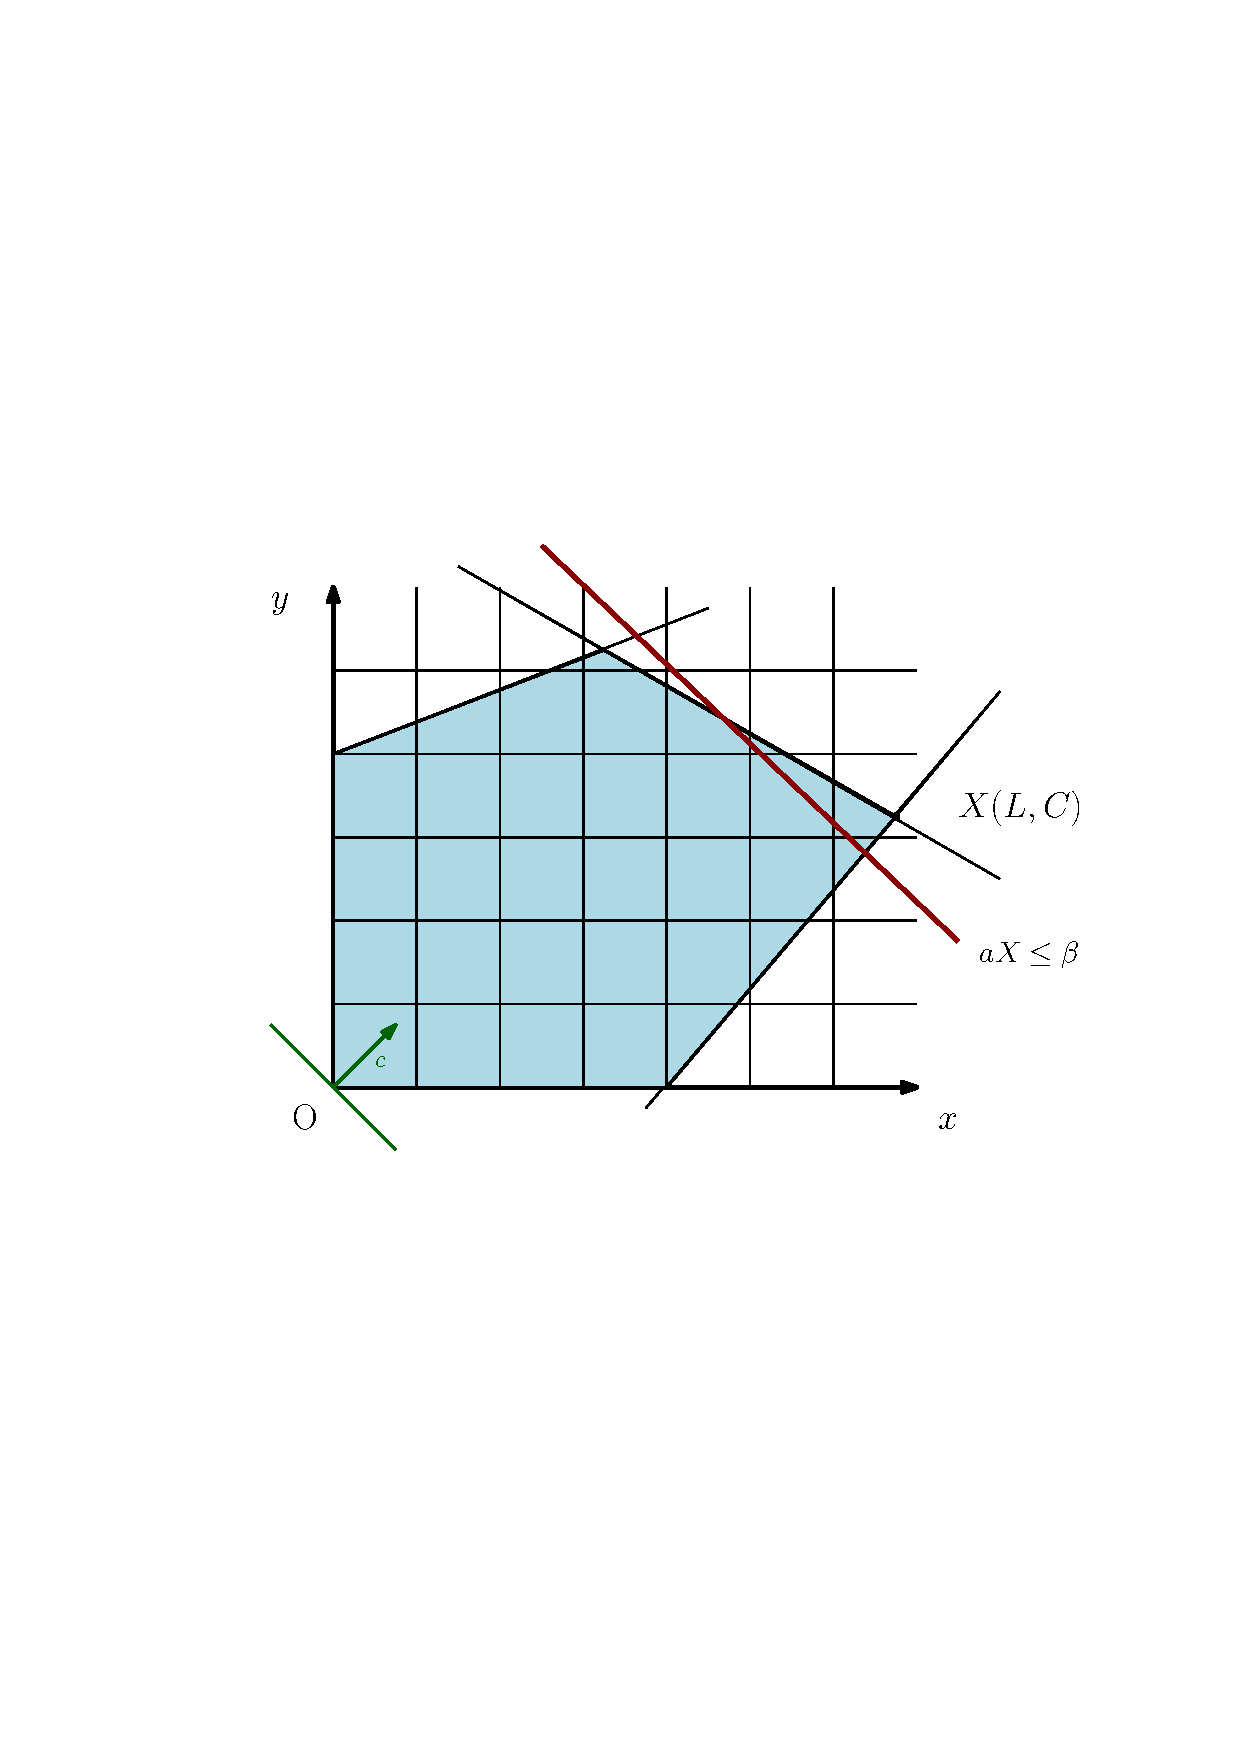
\includegraphics[width=0.8\linewidth]{anh2.pdf}
       
    \end{figure}
    \newpage
\item \textbf{Ý tưởng phương pháp cắt của Danzig}
    
    Việc giải một bài toán $P^N$ là một quá trình gồm nhiều bước:\\
a) Ở bước thứ $r$,  giải bài toán bài toán quy hoạch tuyến tính phụ 
 $P_r, r = 0,1,... 
… \text{với}   F_0=F $\\
b) Tập các điểm  nguyên của tất cả các đa diện lồi là như nhau:
$$F_0^N=F_1^N=F_2^N=...=F_r^N=.......$$\\
Do đó, nếu phương án tối ưu $X^*_r$ của bài toán $P_r$ thoả mãn điều kiện nguyên thì nó cũng là phương án tối ưu $X_0$ của bài toán xuất phát $P^N_0$ và quá trình kết thúc.\\
c)  Nếu $X^*_r$ không thoả mãn điều kiện nguyên thì $X^*_r$ không phải là 
phương án của bài toán $P_{r+1}$, tức là $X_r^*\notin F_{r+1}$.\\Chuyển từ bước $r$ sang bước $r+1$, tức là chuyển từ bài toán $P_r$ sang 
 $P_{r+1}$ khi $X^*_r$ không nguyên được thực hiện nhờ một lát cắt đúng $a_rx \le \beta_r$\\
Việc bổ sung lát cắt này vào ràng buộc của bài toán $P_r$ sẽ chuyển đa diện lồi $F_r$ thành $F_{r+1}$.\\
    
\end{itemize}
\textbf{Nhận xét}
    Phương pháp cắt có hai việc: xấp xỉ tuyến tính đúng nhiều bước đối với bài toán tối ưu nguyên và chuyển từ bước này sang bước khác bằng một lát cắt đúng. Ở đây tồn tại ba vấn đề cần giải quyết: xây dựng một lát cắt đúng, đảm bảo được tính hữu hạn của các bước lặp trong quá trình giải và số lượng lát cắt đúng không được tăng mãi.
    
\subsection{ Thuật toán Gomory cho bài toán tối ưu nguyên hoàn toàn}
Ở phần này, chúng tôi sẽ trình bày về thuật toán và tính hữu hạn của thuật toán Gomory đối với bài toán tối ưu nguyên hoàn toàn và giá trị hàm mục tiêu không nguyên.
\subsubsection{Cơ sở lý thuyết}
Ta xét bài toán tối ưu nguyên hoàn toàn:\\
\begin{equation}\label{Gomory1}
     \begin{split}
      (P^N) \quad    & {\rm{Max}} \langle c,x \rangle\\
          \rm{s.t} &\left\{\begin{split}
            & Ax= b,\\
           & x_j \ge 0, j=1,2,...,n.\\
            & x_j \text{nguyên}, j=1,2..,n.\\
           \end{split}\right.
       \end{split}
   \end{equation}
   \begin{dn}
     Giả  sử hệ véc-tơ $\{A^j,j\in J\}$ là cơ sở tương ứng với phương án cực biên ban đầu của bài toán $P^N$, các véc-tơ $A^j$ và các biến $x_j$ với $j\in J$ được gọi là các véc tơ cơ sở và biến cơ sở; còn các véc-tơ $A^j$ và các biến $x_j$ mà $j \notin J$ được gọi là các véc-tơ tự do và các biến tự do (biến phi cơ sở).\\  
   \end{dn}
    Giả sử $X$ là phương án  tối ưu của bài toán $P^N$, từ đó ta có thể biểu diễn các biến cơ sở qua Các biến phi cơ sở:\\
   \begin{equation}\label{2.4}
       x_{i}=x_{i0} + \sum_{j \in N} x_{ij}(-x_j), i=\overline{0,m}.
   \end{equation}
    Giả sử $x$ là một số thực, ký hiệu $[x]$ là phần nguyên, (số nguyên lớn nhất không vượt quá $x), \{x\}=x-[x]$ là phần lẻ.\\
    VD: $[-1.3]=-2, \{-1.3\}=0.7$.\\
    \begin{dl}
        Giả sử $X$ có $x_{i0}$ không nguyên với $1\le i\le n$ và:\\
        1)\begin{equation}\label{2.5}
            z_i\equiv z_i(X)= -\{x_{i0}\} + \sum_{j \in \mathbb {N} }(-\{x_{ij}\})(-x_{j}), i=\overline{1,n}.
        \end{equation} \\
        2) $x$ là phương án của bài toán $P^N$.\\
        Khi đó:\\
        a)$z_i \hspace{0.1cm} \text{nguyên}$\\
        b) $z_i \ge 0$ 
        \end{dl}

    \begin{hq}
        Giả sử $X(L,C)$ không thoả mãn điều kiện nguyên, như vậy đối 
với $i$ nào đó $(1\le i \le 0) \hspace{0.1cm} x_{i0}$ không nguyên . Khi đó các hệ thức \eqref{2.5}  và $z_i \ge 0$ xác định một lát cắt đúng.
    \end{hq} 
    
    \textbf{Dấu hiệu bài toán không có lời giải:}\\
    -Nếu bài toán $P$ không có lời giải vì hàm mục tiêu không bị chặn trên khúc lồi $F$ thì thuật toán Gomory không áp dụng được.\\
-Thuật toán cũng không áp dụng được cho trường hợp bài toán $P$ có lời giải nhưng $l-\text{bài toán} \overline{P}$ không có lời giải. Điều đó dường như là tập hợp các phương án tối ưu của bài toán $P$ khác trống nhưng không bị chặn.\\
-Về sau ta sẽ giả thiết:\\
1) Hàm mục tiêu $x_0\equiv CX$ bị chặn trên $F$.\\
2) Nếu tập hợp các phương án tối ưu của $P$ khác trống thì nó phải bị chặn, tức là nếu bài toán $P$ giải được thì bài toán $\overline{P}$ cũng giải 
được.\\

\begin{figure}[h]
\centering
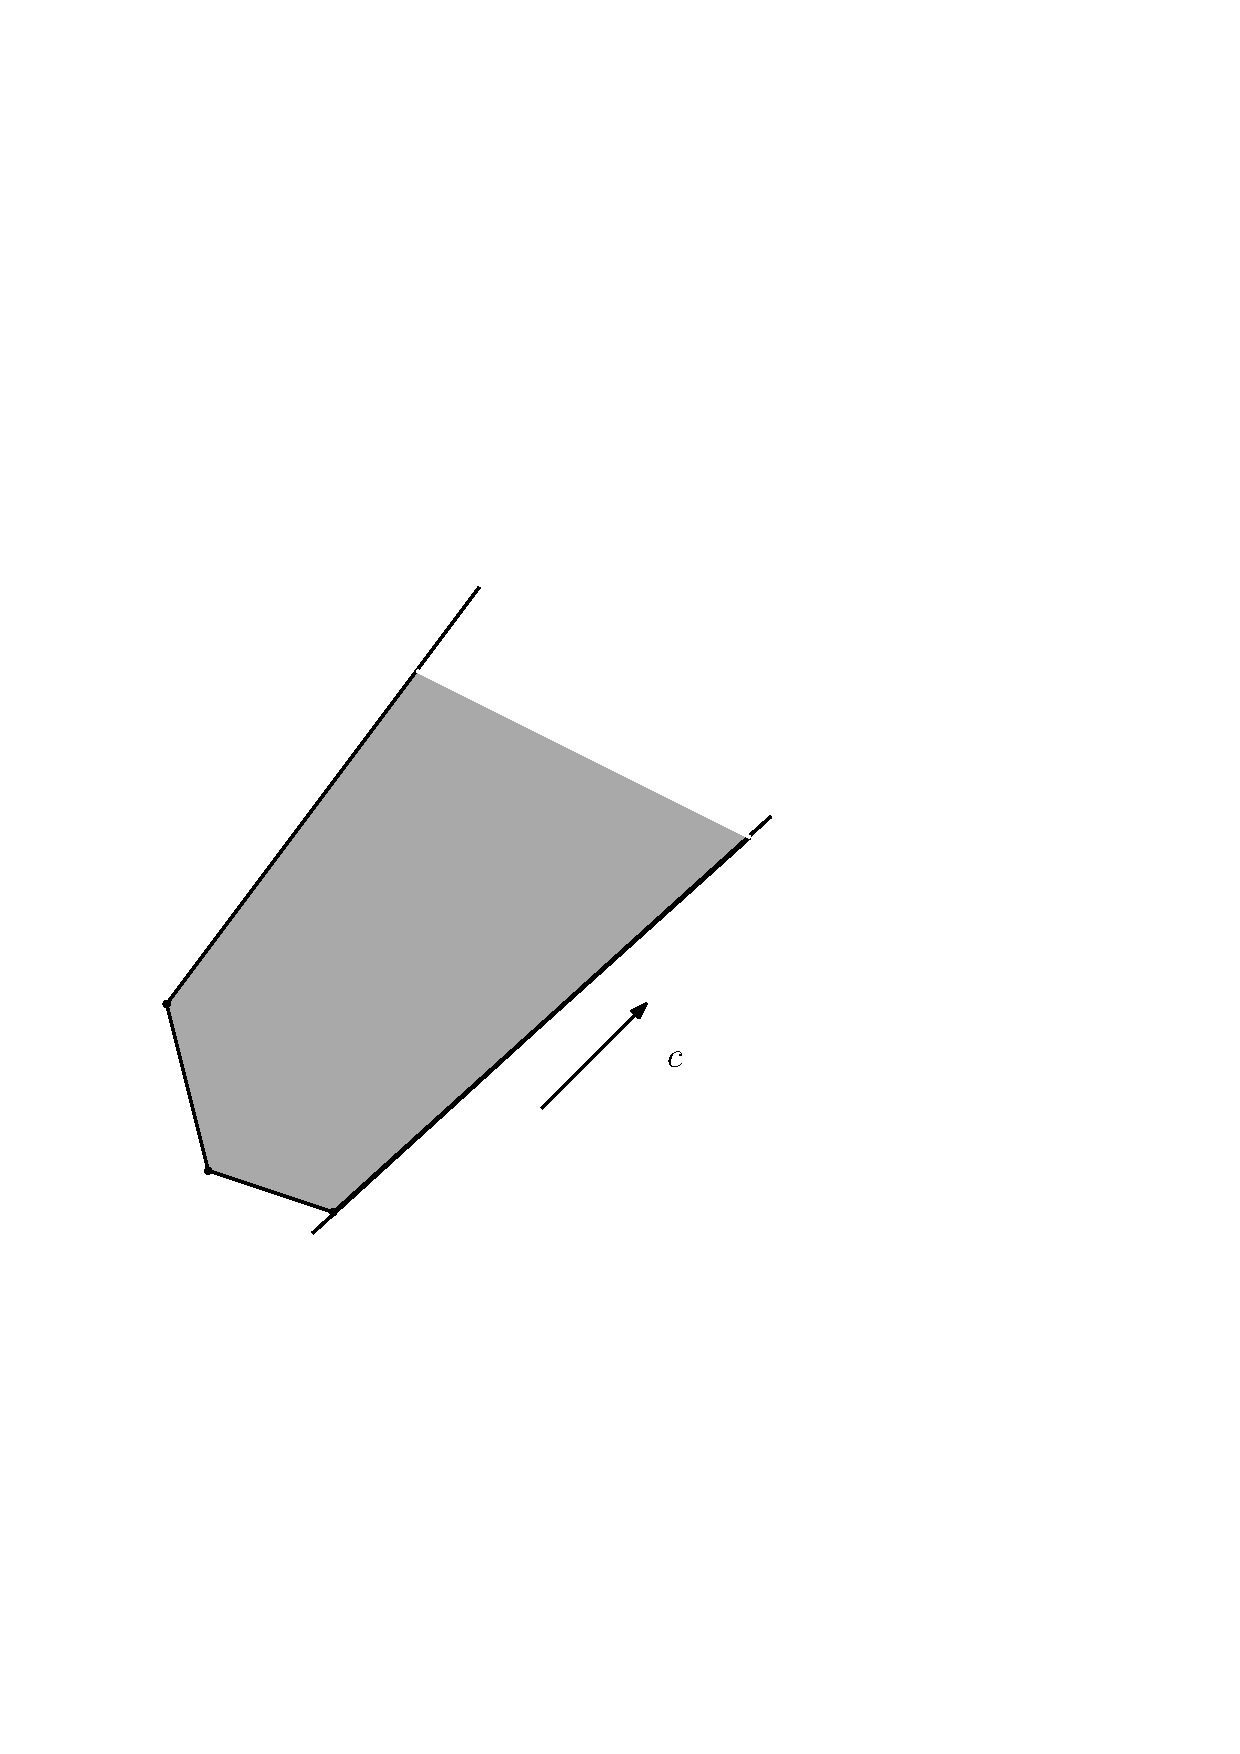
\includegraphics[width=0.3\linewidth]{anh3.pdf}
\caption{$\overline{P}$ không có lời giải}
\end{figure}
\subsubsection{ Thuật toán}

\textbf{Bước 1:}\\
Giải bài toán $P\equiv P_0$ đã cho bằng phương pháp đơn hình đối ngẫu.\\
-Nếu bài toán $P_0$ không giải được thì bài toán $P_0^N$ cũng không giải được.\\
- Nếu bài toán $P$ giải được và nghiệm của nó thỏa mãn điều kiện nguyên thì nó cũng là phương án tối ưu của bài toán $P^N_0$, còn nếu không giải được thì chuyển sang bước 2.\\

\textbf{Bước 2:}
Chọn dòng đầu tiên ứng với thành phần không nguyên:\\
$k=min\{i\|i\in \{1,...,n\},x_{i0}^r \text{không nguyên}\}$ và xây dựng lát cắt đúng:\\
$$   \begin{cases}\label{latcat}
    x_{n+r+1}= -\{x_{k0}^r\} + \sum_{j\in N_r}(-\{x_{kj}^r\} )(-x_j)\\
    x_{n+r+1} \ge 0\\
    x_{n+r+1} \hspace{0.1cm} \text{nguyên}
\end{cases}$$
Ta thêm lắt cắt này vào bảng đơn hình $T_r$, sau đó tiếp tục thực hiện các bước tính toán theo thuật toán đơn hình đối ngẫu từ vựng cho bài toán $P^N_{r+1}$.\\

\textbf{Bước 3:}
Sau khi tính toán với lát cắt nếu được phương án tối ưu thỏa mãn điều kiện nguyên thì thuật toán dừng lại. Nếu không thỏa mãn thì quay lại bước 2 cứ lần lượt như vậy thực hiện các bước lặp $r \ge 0$ cho đến khi thỏa mãn điều kiện.
\textbf{Lưu ý:}\\
Để tránh cho bảng đơn hình không bị có số dòng và cột không xác định, mỗi khi biến phụ tương ứng với lát cắt bị đưa vào cơ sở thì cột tương ứng của nó cũng được xóa khỏi bảng đơn hình.
\subsubsection{Tính hữu hạn của thuật toán:}
\begin{dl}
Giả sử có các điều kiện sau:\\
1) Tính nguyên của hàm mục tiêu $x_0\equiv CX$ được đảm bảo và $x_0$ được xét khi chọn dòng xây dựng lát cắt đúng.\\
2) Một trong các khẳng định sau là đúng:\\
i) Hàm mục tiêu $x_0$ bị chặn dưới trên $F_0$.\\ 
ii) Bài toán $P^N_0$ có ít nhất một phương án $X'$.\\
 Khi đó thuật toán Gomory thứ nhất kết thúc sau một số hữu hạn bước lặp lớn.
 \end{dl}
 
    \subsubsection{Ví dụ}
    \begin{equation*}
        \begin{split}
         &x_1+4x_2 \longrightarrow Max \\
        & \left\{\begin{split}
            & 2x_1+4x_2 \le 7\\
            & 10x_1+3x_2\le 15\\
            & x_1,x_2 \ge 0\\
            & x_1,x_2 \text{nguyên}\\
        \end{split}\right.
    \end{split}
    \end{equation*}
    Ta đưa bài toán về dạng chính tắc. Ta được bài toán mở rộng:\\
    \begin{equation*}
        \begin{split}
         &x_1+4x_2 \longrightarrow Max \\
        & \left\{\begin{split}
            & 2x_1+4x_2+x_3= 7\\
            & 10x_1+3x_2+   x_4= 15\\
            & x_1,x_2,x_3,x_4 \ge 0\\
            & x_1,x_2 \text{nguyên}\\
        \end{split}\right.
    \end{split}
    \end{equation*}
    Ta lập bảng đơn hình:\\
    \begin{center}
        \begin{tabular}{|c|c|c|c|c|c|c|}
    \hline
     Cơ sở & Hệ số & PA& $x_1$ &$x_2$ &$ x_3$ &$x_4$ \\
     \hline
        $x_J$ &$c_J$ &$x_J^0$ &$1$ &$4$ &$0$ &$0$\\
        \hline
        $x_3$ &$0$ &$7$ &$2$ &$4^*$ &$1$ &$0$\\
        $x_4$ &$0$ &$15$ &$10$ &$3$ &$0$ &$1$\\
        \hline
        && $\Delta$ &$-1$ &$-4^*$ &$0$ &$0$\\
        \hline
        $x_2$ &$4$ &$7/4$ &$1/2$ &$1$ &$1/4$ &$0$\\
        $x_4$ &$0$ &$39/4$ &$17/2$ &$0$ &$-3/4$ &$1$\\
        \hline
        && $\Delta$ &$1$ & $0$ &$3$ &$0$\\
        \hline
    \end{tabular}
    \end{center}
    Ta thấy bài toán đã đạt tối ưu nhưng chưa thỏa mãn điều kiện nguyên. Do đó, ta tạo biến $x_5$ theo quy tắc lát cắt Gomory dựa trên biến $x_2$, $$\dfrac{-3}{4}= \dfrac{-1}{2}x_1 -\dfrac{1}{4}x_3 +x_5$$. Ta thêm dòng này vào bảng đơn hình.\\
    \begin{center}
        \begin{tabular}{|c|c|c|c|c|c|c|c|}
        \hline
         Cơ sở & Hệ số & PA& $x_1$ &$x_2$ &$ x_3$ &$x_4$ &$x_5$\\
        \hline
        $x_J$ &$c_J$ &$x_J^0$ &$1$ &$4$ &$0$ &$0$ &$0$\\
        \hline
        $x_2$ &$4$ &$7/4$ &$1/2$ &$1$ &$1/4$ &$0$ &$0$\\
        $x_4$ &$0$ &$39/4$ &$17/2$ &$0$ &$-3/4$ &$1$ &$0$\\
        $x_5$ &$0$ &$-3/4$ &$-1/2^*$ &$0$ &$-1/4$ &$0$ &$1$\\
        \hline
        && $\Delta$ &$1^* $ &$0$ &$1$ &$0$ &$0$\\
        \hline
        $x_2$ &$ 4$ &$1$ &$0$ &$1$ &$0$ &$0$ &$1$\\
        $x-4$ &$0$ &$-3^*$ &$0$ &$0$ &$-5^*$ &$1$ &$17$\\
        $x_1$ & $1$ &$3/2$ &$1$ &$0$ &$1/2$&$0$ &$-2$\\
        \hline
        && $\Delta$ &$0$ &$0$ &$1/2$ &$0$ &$2$\\
        \hline
        $x_2$ &$4$ &$1$ &$0$ &$1$ &$0$ &$0$ &$1$\\
        $x_3$ &$0$ &$3/5$ &$0$ &$0$ &$1$ &$-1/5$ &$-17/5$\\
        $x_1$ &$1$ &$6/5$ &$1$ &$0$ &$1$ &$1/10$&$-3/10$\\
        \hline
        && $\Delta$ &$0$ &$0$ &$0$ &$1/10$ &$37/10$\\
        \hline
        
        \end{tabular}
    \end{center}
    Ta thêm lát cắt mới dựa trên biến $x_1$, 
     $$\dfrac{-1}{5}= \dfrac{-1}{10}x_4 +\dfrac{7}{10}x_5+x_6$$
     \begin{center}
         \begin{tabular}{|c|c|c|c|c|c|c|c|c|}
        \hline
         Cơ sở & Hệ số & PA& $x_1$ &$x_2$ &$ x_3$ &$x_4$ &$x_5$ &$x_6$\\
        \hline
        $x_J$ &$c_J$ &$x_J^0$ &$1$ &$4$ &$0$ &$0$ &$0$ &$0$\\
        \hline
        $x_2$ &$4$ &$1$ &$0$ &$1$ &$0$ &$0$ &$1$ &$0$\\
        $x_3$ &$0$ &$3/5$ &$0$ &$0$ &$1$ &$-1/5$ &$-17/5$ & $0$\\
        $x_1$ &$1$ &$6/5$ &$1$ &$0$ &$1$ &$1/10$&$-3/10$ &$0$\\
        $x_6$ &$0$ &$-1/5$ &$0$ &$0$ & $0$ &$-1/10^*$ &$7/10$ &$1$\\
        \hline
        && $\Delta$ &$0$ &$0$ &$0$ &$1/10$ &$37/10$ &$0$\\
        \hline
        $x_2$ &$4$ &$1$ &$0$ &$1$ &$0$ &$0$ &$1$ &$0$\\
        $x_3$ &$0$ &$1$ &$0$ &$0$ &$1$ &$0$ &$-24/5$ &$-2$\\
        $x_1$ &$1$ &$1$ &$1$ &$0$ &$0$ &$0$ &$2/5$ &$1$\\
        $x_4$ &$0$ &$2$ &$0$ &$0$ &$0$ &$1$ &$-7$ &$-10$\\
        \hline
        && $\Delta$ &$0$ &$0$ &$0$ &$0$&$ 22/5$ &$1$\\
        \hline
        
         \end{tabular}
     \end{center}
     Bài toán đã đạt tối ưu đồng thời thỏa điều kiện nguyên nên ta dừng thuật toán và kết luận được $x=(x_1,x_2)=(1,1)$ và giá trị hàm mục tiêu là $5$.
\subsection{Thuật toán Gomory cho bài toán tối ưu nguyên bộ phận}
 Đối với bài toán tối ưu nguyên bộ phận ta có tất cả các lý thuyết cơ sở cũng như thuật toán tương tự như ở bài toán tối ưu nguyên hoàn toàn.Tuy nhiên, ở việc chọn dòng để hình thành lát cắt:
 $k=min\{i|i\in \{1,...,n\},x_{i0}^r \text{không nguyên}\}$, trong đó ta chỉ xét trên các biến mà đề bài bắt buộc nguyên, và trực tiếp bỏ qua các biến không có điều kiện nguyên.
 \subsubsection{Ví dụ}
 Ta xét bài toán sau:
 \begin{equation*}
        \begin{split}
         & 4x_1+5x_2+3x_3\longrightarrow Max \\
        & \left\{\begin{split}
            & 3x_1+   +4x_3 \le 10\\
            & 2x_1+x_2+x_3 \le 7\\
            & 3x_1+4x_2+x_3 \le 12\\
            & x_1,x_2,x_3 \ge 0\\
            & x_1,x_3 \text{nguyên}\\
        \end{split}\right.
    \end{split}
    \end{equation*}
    Ta đưa bài toán về dạng chính tắc:\\
    \begin{equation*}
        \begin{split}
         &4x_1+5x_2+3x_3 \longrightarrow Max \\
        & \left\{\begin{split}
            & 3x_1+  +4x_3+x_4=10\\
            &2x_1+x_2+x_3+x_5=7\\
            &3x_1+4x_2+x_3+  x_6=12\\
            & x_1,x_2,x_3,x_4,x_4,x_6 \ge 0\\
            & x_1,x_3 \text{nguyên}\\
        \end{split}\right.
    \end{split}
    \end{equation*}
    \begin{center}
        \begin{tabular}{|c|c|c|c|c|c|c|c|c|}
        \hline
         Cơ sở & Hệ số & PA& $x_1$ &$x_2$ &$x_3$ &$x_4$ &$x_5$ &$x_6$  \\
         \hline
          $x_J$& $c_J$ &$x_J^0$ &$4$ &$5$ &$ 3$ &$0$ &$0$ &$0$\\
          \hline
          $x_4$ &$0$ &$10$ &$3$ &$0$ &$4$ &$1$ &$0$ &$0$\\
          $x_5$ &$0$ &$7$ &$2$ &$1$ &$1$ &$0$ &$1$ &$0$\\
          $x_6$ &$0$ &$12$ &$3$ &$4^*$ &$1$ &$0$ &$0$ &$1$\\
          \hline
          &&$\Delta$ &$-4$ &$-5$ &$-3$ &$0$ &$0$ &$0$\\
          \hline
      \end{tabular}
    \end{center}    
    \begin{center}
        \begin{tabular}{|c|c|c|c|c|c|c|c|c|}
        \hline
          Cơ sở & Hệ số & PA& $x_1$ &$x_2$ &$x_3$ &$x_4$ &$x_5$ &$x_6$  \\
         \hline
          $x_J$& $c_J$ &$x_J^0$ &$4$ &$5$ &$ 3$ &$0$ &$0$ &$0$\\
          \hline    
          $x_4$ & $0$ &$10$ &$3$ &$0$ &$4^*$ &$1$ &$0$ &$0$ \\
          $x_5$ &$0$ &$4$ &$5/4$ &$0$ &$3/4$ &$0$ &$1$ &$-1/4$\\
          $x_2$ &$5$ &$3$ &$3/4$ &$1$ &$1/4$ &$0$ &$0$ &$1/4$\\
          \hline
          &&$\Delta$ &$-1/4$ &$0$ &$-3^*$ &$0$ &$0$ &$5/4$\\
          \hline
          $x_3$ &$3$ &$5/2$ &$3/4$ &$0$ &$1$ &$1/4$ &$0$ &$0$\\
          $x_5$ &$0$ &$17/8$ &$11/16$ &$0$ &$0$ &$-3/16$ &$0$ &$-1/4$\\
          $x_2$ &$5$ &$19/8$ &$9/16$ &$1$ &$0$ &$-1/16$ &$1$ &$1/4$\\
          \hline
          &&$\Delta$ &$17/16$ &$0$ &$0$ &$7/16$ &$0$ &$5/4$\\
          \hline
         \end{tabular}
    \end{center}
    Lúc này bài toán đạt tối ưu nhưng chưa thỏa điều kiện nguyên, ta xét biến $x_3$ để tạo lát cắt Gomory, bỏ qua $x_2$ vì đề bài chỉ yêu cầu $x_1,x_3$ phải nguyên.
    $$\dfrac{-1}{2}=\dfrac{-3}{4}x_1 -\dfrac{1}{4}x_4 +x_7$$.
    \begin{center}
        \begin{tabular}{|c|c|c|c|c|c|c|c|c|c|}
        \hline
         Cơ sở & Hệ số & PA& $x_1$ &$x_2$ &$x_3$ &$x_4$ &$x_5$ &$x_6$ &$x_7$ \\
         \hline
          $x_J$& $c_J$ &$x_J^0$ &$4$ &$5$ &$ 3$ &$0$ &$0$ &$0$ &$0$\\
          \hline
           $x_3$ &$3$ &$5/2$ &$3/4$ &$0$ &$1$ &$1/4$ &$0$ &$0$ &$0$\\
          $x_5$ &$0$ &$17/8$ &$11/16$ &$0$ &$0$ &$-3/16$ &$0$ &$-1/4$ &$0$\\
          $x_2$ &$5$ &$19/8$ &$9/16$ &$1$ &$0$ &$-1/16$ &$1$ &$1/4$ &$0$\\
          $x_7$ &$0$ &$-1/2$ &$-3/4$ &$0$ &$0$ &$-1/4^*$ &$0$ &$0$ &$1$\\
          \hline
          &&$\Delta$ &$17/16$ &$0$ &$0$ &$7/16$ &$0$ &$5/4$ &$0$\\
          \hline
          $x_3$ &$3$ &$2$ &$3/4$ &$0$ &$1$ &$0$ &$0$ &$0$ &$1$\\
          $x_5$ &$0$ &$5/2$ &$5/4$ &$0$ &$0$ &$0$ &$1$ &$-1/4$ &$-3/4$\\
          $x-2$ &$5$ &$5/2$ &$3/4$ &$1$ &$0$ &$0$ &$0$ &$1/4$ &$-1/4$\\
          $x_4$ &$0$ &$2$ &$3^*$ &$0$ &$0$ &$1$ &$0$ &$0$ &$-4$\\
          \hline
          &&$\Delta$&$-1/4$ &$0$ &$0$ &$0$ &$0$ &$5/4$ &$7/4$\\
          \hline
          \end{tabular}
    \end{center}    
    \begin{center}
        \begin{tabular}{|c|c|c|c|c|c|c|c|c|c|}
        \hline
          Cơ sở & Hệ số & PA& $x_1$ &$x_2$ &$x_3$ &$x_4$ &$x_5$ &$x_6$ &$x_7$ \\
         \hline
          $x_J$& $c_J$ &$x_J^0$ &$4$ &$5$ &$ 3$ &$0$ &$0$ &$0$ &$0$\\
          \hline
          $x_3$ &$3$ &$2$ &$0$ &$0$ &$1$ &$0$ &$0$ &$0$ &$1$\\
          $x_5$ &$0$ &$5/3$ &$0$ &$0$ &$0$ &$5/12$ &$1$ &$-1/4$ &$11/2$\\
          $x_2$ &$5$ &$2$ &$0$ &$1$ &$0$ &$-1/4$ &$0$ &$1/4$ &$3/4$\\
          $x_1$ &$4$ &$2/3$ &$1$ &$0$ &$0$ &$1/3$ &$0$ &$0$ &$-4/3$\\
          \hline
          &&$\Delta$ &$0$ &$0$ &$0$ &$1/12$ &$0$ &$5/4$ &$17/12$\\
          \hline
        \end{tabular}
    \end{center}
    Ta xét $x_1$ và lập lát cắt mới, $\dfrac{-2}{3}= \dfrac{-1}{3}x_4 +\dfrac{1}{3}x_7+x_8$.
    \begin{center}
        \begin{tabular}{|c|c|c|c|c|c|c|c|c|c|c|}
        \hline
          Cơ sở & Hệ số & PA& $x_1$ &$x_2$ &$x_3$ &$x_4$ &$x_5$ &$x_6$ &$x_7$&$x_8$ \\
         \hline
          $x_J$& $c_J$ &$x_J^0$ &$4$ &$5$ &$ 3$ &$0$ &$0$ &$0$ &$0$ &$0$\\
          \hline
           $x_3$ &$3$ &$2$ &$0$ &$0$ &$1$ &$0$ &$0$ &$0$ &$1$ &$0 $\\
          $x_5$ &$0$ &$5/3$ &$0$ &$0$ &$0$ &$5/12$ &$1$ &$-1/4$ &$11/2$ &$0$\\
          $x_2$ &$5$ &$2$ &$0$ &$1$ &$0$ &$-1/4$ &$0$ &$1/4$ &$3/4$ &$0$\\
          $x_1$ &$4$ &$2/3$ &$1$ &$0$ &$0$ &$1/3$ &$0$ &$0$ &$-4/3$ &$0$\\
          $x_8$ &$0$ &$-2/3$ &$0$ &$0$ &$0$ &$-1/3^*$ &$0$ &$0$ &$1/3$ &$1$\\
          \hline
          &&$\Delta$ &$0$ &$0$ &$0$ &$1/12$ &$0$ &$5/4$ &$17/12$ &$0$\\
          \hline
          $x_3$ &$3$ &$2$ &$0$ &$0$ &$1$ &$0$ &$0$ &$1$ &$0$& $0$\\
          $x_5$ &$0$ &$5/6$ &$0$ &$0$ &$0$ &$0$ &$1$ &$-1/4$ &$71/12$ &$5/4$\\
          $x_2$ &$5$ &$5/2$ &$0$ &$1$ &$0$ &$0$ &$0$&$1/4$ &$1/2$ &$-3/4$\\
          $x_1$ &$4$ &$0$ &$1$ &$0$ &$0$ &$0$ &$0$ &$0$ &$-1$ &$1$\\
          $x_4$ &$0$ &$2$ &$0$ &$0$ &$0$ &$1$ &$0$ &$0$ &$-1$ &$-3$\\
          \hline
          &&$\Delta$ &$0$ &$0$ &$0$ &$0$ &$0$ &$5/4$ &$3/2$ &$1/4$\\
          \hline
        \end{tabular}
    \end{center}
    Ta dừng thuật toán và kết luận nghiệm của bài toán đã cho là $x=(x_1,x_2,x_3)=(0,\dfrac{5}{2},2)$ và giá trị tối ưu của hàm mục tiêu là $18.5$.








































































    
\subsection{Ý nghĩa của phương pháp Gomory}

\section{Phương pháp Land-Doig}

\subsection{Giới thiệu phương pháp và ý nghĩa}

\subsection{Các bước thực hiện của phương pháp}

\subsection{Ví dụ minh họa}

\chapter{Mở rộng kết quả cho bài toán dạng phân thức tuyến tính}


\chapter*{Kết luận}                         % Chương 3
\addcontentsline{toc}{chapter}{{\bf  Kết luận}\rm}
\indent
\thispagestyle{fancy}

Luận văn này đạt được các vấn đề sau đây:

\begin{itemize}
	\item  Giới thiệu bài toán tối ưu nguyên.
	\item  Trình bày về tư tưởng lát cắt và thuật toán của Gomory để giải bài toán Tối ưu tuyến 
	\item
\end{itemize}



\begin{thebibliography}{99}
	\addcontentsline{toc}{chapter}{{\bf  Tài liệu tham khảo}} 
	\thispagestyle{fancy}
%	\item[\textbf{\large 1.}] \textbf{\large Tài liệu tham khảo chính thức}
	
	%\item[\textbf{\large 1.}] \textbf{\large Tài liệu tham khảo chính thức}
	
	
	%Các tài liệu chính được tôi chọn lựa để tham khảo khi thực hiện luận văn là  tài liệu số \cite{Mat}, \cite{Gab1} và \cite{Gian}. 	Các vấn đề liên quan được chúng tôi khảo cứu trong các tài liệu còn lại.
	
	\bibitem{Erik} Erik B. Bajanilov, {\it Linear fractional programming: Theory, Mẹthods, Applications, and Software}, Springer, 2003.
		
	\bibitem{Stan} Stancu Minasian, {\it Fractional Programming: Theory, Methods, and Applications}, Kluwer Academic Publishers, 1992.
	

	
	
\end{thebibliography}

\end{document}